\documentclass[titlepage]{article}
\usepackage[english]{babel}
\usepackage[utf8]{inputenc}
\usepackage{fancyhdr}
\usepackage{amsfonts} 
\usepackage{amsmath}
\usepackage{glossaries}
\usepackage[colorlinks]{hyperref}
\usepackage{venndiagram}
\usepackage{tikz}

\pagestyle{fancy}
\fancyhf{}
\rhead{Joshua Murphy}
\lhead{Course Notes - COMP 1002}
\rfoot{Page \thepage}
\title{COMP 1002 Survival Guide}
\author{Joshua Murphy}
\date{\today}
\newglossaryentry{implication}{%
  name={Implication},%
  description={valid knowledge used to refer to an area of human endeavour, an autonomous computer activity, or other specialized discipline}}

\newglossaryentry{set-builder-notation}{%
  name={Set Builder Notation},%
  description={A form of mathematical notation to denote a range of numbers
instead of writing them out individually. Follows the format $ \{x \in
\mathbb{R} | y \leq x \leq z\} $}}

\newglossaryentry{set}{%
  name={Set},%
  description={A collection of objects}}


\makeglossaries
\begin{document}
\maketitle
\tableofcontents{}
\pagebreak


% Begin section on propositional logic 
\section{Propositional Logic}


\subsection{Implication}
In logic, an \gls{implication} is a 


\begin{equation}p \to q \end{equation}
This is read as ``\textit{p implies q.}'' In this case $P$ = it is raining, 
and $Q$ = there are clouds. 
Insert truth table
\subsubsection{Example:}
$p \to q$
\subsection{Biconditional}
\begin{equation}
p \iff q \end{equation}
This is read as ``\textit{p if and only if q.}'' Both $P$ and $Q$ must be the
same value. This differs from $\wedge$ in which both values must be
\textit{true.} For example, $P$ = taking a flight and $Q$ = buying a ticket. It
is false when they have opposite values. You can take the flight if and only if
you buy a ticket.

$\equiv \in \notin \emptyset \forall \exists \rightarrow \leftrightarrow \sigma
\psi \phi $



% Begin section of Predicates, quantifiers and sets.
\section{Predicates, Quantifiers, Sets}
\subsection{Sets}


\subsection{Predicates}
Contradiction: False all the time

Satisfiable: True if it's true at least once.

Valid: True all the time

A \gls{set} is a collection of objects. 
\subsubsection{Set Builder Notation}
\gls{set-builder-notation} is a form of mathermatical notation to describe a
range of values without having to write each number out individually. For
example, instead of saying $\mathbb{S} = \{1, 2, 3, 4, 5, 6, 7, 8, 9, 10 \}$ we
can say $\{\mathbb{S} = { x \in \mathbb{R} | 1 \leq x \leq 10}\}$ in order to
denote the same thing, but in set builder notation.

\subsubsection{Types of Common Sets}
$ \emptyset $ denotes the empty set\\
$ \mathbb{S} = \{1, 2, 3\}$ denotes the set containing 1, 2, and 3. \\  
$ \mathbb{N} = \{ 1,3,3\cdots\}$  is the set of \textit{natural} numbers.
Usually starts at 1 \\
$ \mathbb{Z} = \{\cdots, -2, -1, 0, 1, 2 \cdots\} $ is the set of integers,
which can be negative \\
\newline So, on forth  for real numbers, complex, rational, etc. You can also
create your own sets with whatever names or letters you wish, and in questions
you'll see sets containing any sort of values representing any kind of
category. If you are a programmer, you can think of them like arrays.

\subsubsection{Set Elements}

Means that element $a$ is in set S: 
\begin{equation}
 a \in S 
\end{equation}
Means $a$ is not in S:
\begin{equation}
 a \notin S
\end{equation}
\newline Susan is not a bankteller, i.e  Susan $\notin$ Banktellers: \newline
\newline 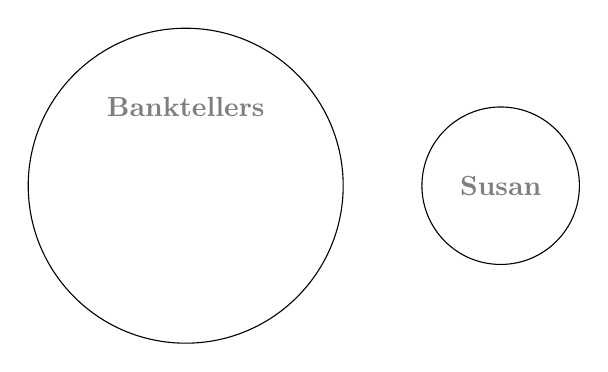
\begin{tikzpicture} 
    \begin{scope}[shift={(0cm,-2cm)}, fill opacity=0.5]
        \draw[fill=white, draw = black] (-1.5,0) circle (2);
        \draw[fill=white, draw = black] (2.5,0) circle (1);
    \node at (-1.5,1) (A) {\textbf{Banktellers}};
    \node at (2.5,0) (B) {\textbf{Susan}};
    \end{scope}
\end{tikzpicture} \\
\newline Susan is a bankteller, i.e Susan $\in$ Banktellers: \newline
\newline 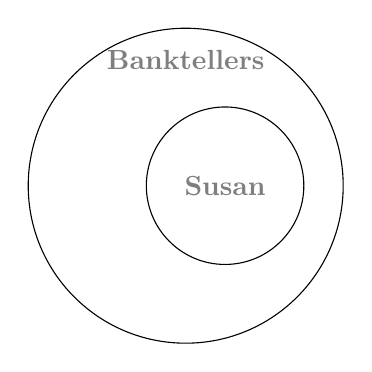
\begin{tikzpicture}
    \begin{scope}[shift={(0cm,-2cm)}, fill opacity=0.5]
        \draw[fill=white, draw = black] (-1.5,0) circle (2);
        \draw[fill=white, draw = black] (-1,0) circle (1);
    \node at (-1.5,1.6) (A) {\textbf{Banktellers}};
    \node at (-1,0) (B) {\textbf{Susan}};
    \end{scope}
\end{tikzpicture} \\

\subsubsection{Operations on Sets}
Intersection: $ A \cap B = \{ x \mid x \in A \wedge x \in B\}$ \\
\begin{venndiagram2sets}
    \fillACapB
\end{venndiagram2sets} \\
Union : $A \cup B = \{ x \mid x \in A \vee x \in B\}$ \\
\begin{venndiagram2sets}
    \fillA \fillB
\end{venndiagram2sets}
Set Difference : $A \setminus B = \{ x \mid x \in A \wedge x \notin B\}$ \\
\begin{venndiagram2sets}
    \fillA \fillB
\end{venndiagram2sets}
Symmetric Difference : $A \Delta B = \{ (A - B) \cup (B - A) \}$ \\
\begin{venndiagram2sets}
    \fillANotB
\end{venndiagram2sets}
Complement: $ \bar{A} = \{ x \in U \mid x \notin A \}$ \\
Subset: $ A \subset B $ \\
Proper Subset: $ A \subseteq B $


% Import rest of sections here . . . 
% \include{cool}

\printglossaries
\end{document}
